\documentclass[a4paper, 12pt]{article}

%Paragraph jumps and indentation
\setlength{\parskip}{1.5em}
\setlength{\parindent}{1.25cm}

%Border
\usepackage[left=1in, right=1in, top=1in, bottom=1in]{geometry}

%Double spacing
\usepackage{setspace}
\doublespacing

%Packages
\usepackage{amsmath}
\usepackage[dvipsnames]{xcolor}
\usepackage{mathtools}
\usepackage{amsfonts}
\usepackage{titlesec}

%Images
\usepackage{graphicx}
\graphicspath{ {./images/} }
\usepackage{wrapfig}
\usepackage{float}

%Tables
\usepackage{multirow}
\usepackage{array}
\usepackage{tabu}
\titleformat{\section}
{\normalfont\large\bfseries}{\thesection}{1em}{}
\titleformat{\subsection}
{\normalfont\large\bfseries}{\thesubsection}{1em}{}

%Equation numbering
\counterwithin{equation}{section}

%Links
\usepackage{hyperref}
\urlstyle{same}

%Diagrams
\usepackage{pgfplots}
\pgfplotsset{compat = newest}
\usetikzlibrary{positioning, arrows.meta}
\usepgfplotslibrary{fillbetween}
\usepackage{wrapfig}


\begin{document}

\begin{titlepage}
  \begin{center}
    \textbf{IB ECONOMICS} \hspace{1cm} STANDARD LEVEL\\
    \vspace*{3cm}
    \textbf{Title of the article:}
    Yle budget cuts agreed after Left,
    Greens and Finns Party approve new deal\\

    \textbf{Source of the article:}
    Yle News\\

    \textbf{Link to the article:}
    \url{https://yle.fi/a/74-20111279}\\

    \textbf{Article publish date:}
    September 12, 2024\\

    \textbf{Commentary writing date:} \today\\

    \textbf{Unit of the syllabus:}
    Microeconomics\\

    \textbf{Key concept:}
    Economic Well-Being.\\

    \vfill
    Word count: 069
  \end{center}
\end{titlepage}

\section*{Extract}
{ \itshape
  {\large The deal means that Yle faces a funding freeze and an increase in VAT payments, after a long drawn-out battle over setting the company's spending limits up to 2027.}

  Yle faces a years-long funding freeze after parliamentary parties agreed a deal on the company's budget, with the Finns Party, Greens and Left Alliance all approving the new agreement.

  The deal will freeze the budget until 2027, and increase the VAT rates levied on the company from 10 percent to 14 percent from 2026. Yle's budget in 2027 will be around 47 million euros smaller than it would be if index-linked budget increases occurred annually.

  The company will also be obliged to increase commissioning from external production companies, with external purchases slated to be around 15-20 percent higher than they were in the period 2021-2023.

  In addition, Yle will be required to publish more information about its activities and spending.

  The company is owned by the Finnish state and funded by a tax that in 2024 was a maximum of 163 euros per year for individual taxpayers, with reductions for those on lower incomes, or 3,000 euros for businesses.

  Parties have been at loggerheads over Yle's budget since the election campaign, in which both the National Coalition and Finns Party argued for cuts worth more than a hundred million euros in Yle's funding.
}
\newpage
\textbf{\textit{\large Consusus decision}}\\
{ \itshape

  Yle's budget is traditionally decided by cross-party consensus, separate to the government programme. This is regarded as a safeguard against politicising the public service media company, but this time around negotiations were difficult and protracted.

  National Coalition MP Matias Marttinen chaired the working group seeking a compromise, with his own party and the Finns Party suggesting that the government could take the decision themselves if cross-party consensus wasn't reached.

  In July a proposal was accepted by all the parliamentary parties except the Greens and the Left Alliance, who were annoyed at the way the proposal had been negotiated between the Finns Party and National Coalition, rather than between all the parties in the working group.

  The two parties secured small changes to the text of the deal, relating to working conditions of staff and reinforced a commitment to the production of high quality programming for children and young people, and its role as a pillar of general education and a guarantor of equality in educational equality.

  The Movement Now party, a one-man group consisting of Apprentice presenter Harry Harkimo, announced early on that it would reject the agreement on Yle funding.
}

\includegraphics{Screenshot 2025-01-20 131959.png}

\newpage

\section*{Commentary}

The article celebrates the conclusion of discussions within the government regarding the funding of Yle, the Finnish Public Service Media Company.
Consensus is reached after much deliberation, and consequently the budget of Yle will be reduced both directly by reducing the direct tax "yleisradiovero" and indirectly through the funding freeze and the VAT increase.
This commentary aims to analyse the effects of the changes by simplifying the situation and treating it as a reduction of specific subsidy granted to the company.
It will be shown that this change successfully advances \textbf{\color{orange}{economic well-being}}, around which the discussion will revolve.

One of the motivations for the government running Yle is to attempt to correct the allocative inefficiency caused by positive consumption externalities, which arise from gererally accessible news making the Finnish population more aware.
An equally important reason for it, however, is increasing \textbf{\color{orange}{equity}} in the Finnish society.
Therefore, it is a fundamental principle of the company to keep their services free for all consumers.
\begin{wrapfigure}{L}{0.6\textwidth}
  \begin{center}
    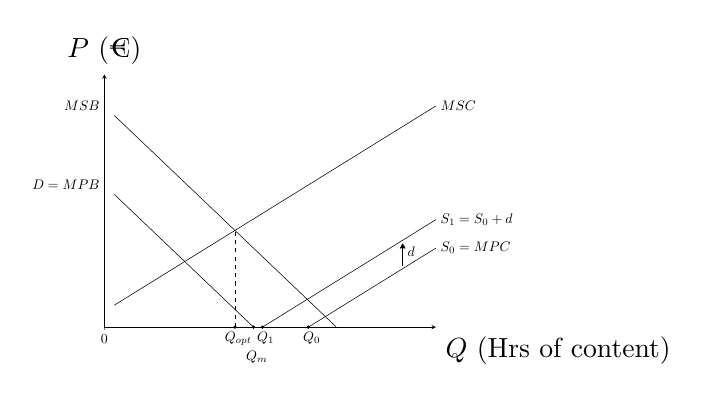
\begin{tikzpicture}[scale=0.5]
      \begin{axis}[
          width=10cm,
          height=8cm,
          axis lines = left,
          xtick = {0},
          ytick = {\empty},
          xmin = 0, xmax = 10,
          ymin = 0, ymax = 8,
          clip = false
        ]
        % Supply curves
        \addplot[domain = 0.3:10, restrict y to domain = 0:8, samples = 400]{0.65*x+0.5};
        \addplot[domain = 0.3:10, restrict y to domain = 0:8, samples = 400]{0.65*x-3.1};
        \addplot[domain = 0.3:10, restrict y to domain = 0:8, samples = 400]{0.65*x-4};

        % Demand curves
        \addplot[domain = 0.3:10, restrict y to domain = 0:8, samples = 400]{-x+4.5};
        \addplot[domain = 0.3:10, restrict y to domain = 0:8, samples = 400]{-x+7};

        % D/S curve labels
        \node[right] at (10, 7) {$MSC$};
        \node[right] at (10, 3.4) {$S_1=S_0 + d$};
        \node[right] at (10, 2.5) {$S_0=MPC$};

        \node[left] at (0, 4.5) {$D=MPB$};
        \node[left] at (0, 7) {$MSB$};

        \draw[dashed] (3.939, 0) -- (3.939, 3.060);
        \filldraw[black] (3.939, 0) circle (1pt);
        \node[below] at (4.039, 0) {$Q_{opt}$};

        \filldraw[black] (4.5, 0) circle (1pt);
        \node[below] at (4.6, -0.6) {$Q_m$};

        \filldraw[black] (4.769, 0) circle (1pt);
        \node[below] at (4.869, 0) {$Q_1$};

        \filldraw[black] (6.154, 0) circle (1pt);
        \node[below] at (6.254, 0) {$Q_0$};

        \draw[-Triangle] (9, 1.95) to (9, 2.65);
        \node[right] at (9, 2.4) {$d$};



      \end{axis}
      \node[below right] at (current axis.right of origin) {$Q \text{ (Hrs of content)}$};
      \node[above] at (current axis.above origin) {$P \text{ (\texteuro)}$};
    \end{tikzpicture}
    \caption{Effects of the Budget Cut to Yle's Supply}
  \end{center}
\end{wrapfigure}

\textbf{Figure 1} displays the effects of the new legislation with reference to the supply of content produced by Yle.
The curves $S_0$ and $S_1$ represent the supply before and after the budget is cut by some amount $d$ for every unit of output. 
Consequently, the amount of content that is produced by Yle is reduced from $Q_0$ to $Q_1$, thanks to the stricter budget.
The quantity is still greater than that represented by the point $Q_m$, which shows the amount of content that the population of Finland is willing and able to consume.
This means that the change is only able to reduce the amount of surplus content from $Q_0-Q_m$ to $Q_1-Q_m$.

The principle of keeping the services of Yle free of charge for everyone can be treated as a price ceiling of $0$€.
In the status quo illustrated by line $S_1$ in \textbf{Figure 1}, the price ceiling has no effect and there will be no shortage of content.
However, attempting to reach allocative efficiency by adjusting the budget of Yle would be practically impossible without creating either a surplus or a shortage.
This issue is due to the difference between the quantity of content needed for allocative efficiency $Q_{opt}$, and the quantity demanded by the market $Q_m$.
Neither of these quantities can be affected by adjusting the budget of Yle:
The former is the target amount of content the government aims to produce by adjusting the size of the budget, while the latter is the amount of content that the population is willing and able to consume for free.

\begin{wrapfigure}{L}{0.6\textwidth}
  \begin{center}
    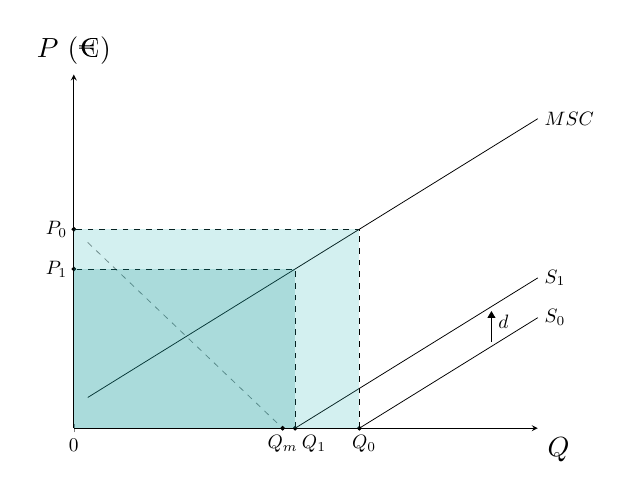
\begin{tikzpicture}[scale=0.7]
      \begin{axis}[
          width=10cm,
          height=8cm,
          axis lines = left,
          xtick = {0},
          ytick = {\empty},
          xmin = 0, xmax = 10,
          ymin = 0, ymax = 8,
          clip = false
        ]
        % Supply curves
        \addplot[domain = 0.3:10, restrict y to domain = 0:8, samples = 400]{0.65*x+0.5};
        \addplot[domain = 0.3:10, restrict y to domain = 0:8, samples = 400]{0.65*x-3.1};
        \addplot[domain = 0.3:10, restrict y to domain = 0:8, samples = 400]{0.65*x-4};

        % MPB
        \draw[gray, dashed] (0.3, 4.2) -- (4.5, 0);

        % Supply curve labels
        \node[right] at (10, 7) {$MSC$};
        \node[right] at (10, 3.4) {$S_1$};
        \node[right] at (10, 2.5) {$S_0$};


        % Orange rectangle
        \filldraw[black] (4.769, 0) circle (1pt);
        \node[below right] at (4.769, 0) {$Q_1$};
        \filldraw[black] (0, 3.6) circle (1pt);
        \node[left] at (0, 3.6) {$P_1$};

        \draw[dashed] (4.769, 0) -- (4.769, 3.6) -- (0, 3.6);
        \fill[teal, opacity = 0.2] (0, 0) -- (4.769, 0) -- (4.769, 3.6) -- (0, 3.6);


        % Pink rectangle
        \filldraw[black] (6.154, 0) circle (1pt);
        \node[below] at (6.254, 0) {$Q_0$};
        \filldraw[black] (0, 4.5) circle (1pt);
        \node[left] at (0, 4.5) {$P_0$};

        \draw[dashed] (6.154, 0) -- (6.154, 4.5) -- (0, 4.5);
        \fill[TealBlue, opacity = 0.2] (0, 0) -- (6.154, 0) -- (6.154, 4.5) -- (0, 4.5);

        \draw[-Triangle] (9, 1.95) to (9, 2.65);
        \node[right] at (9, 2.4) {$d$};

        % Q_m
        \filldraw[black] (4.5, 0) circle (1pt);
        \node[below] at (4.5, 0) {$Q_m$};


      \end{axis}
      \node[below right] at (current axis.right of origin) {$Q$};
      \node[above] at (current axis.above origin) {$P \text{ (\texteuro)}$};
    \end{tikzpicture}
    \caption{Consequent Change to Govt. Expenditure}
  \end{center}
\end{wrapfigure}

\noindent \textbf{Figure 2} highlights the reduction in government expenditure as a result of this change.
The amount of money that the government saves thanks to this change can be calculated: \\
$(Q_0-Q_1)\cdot (P_0-P_1) = (Q_0-Q_1)\cdot d$\\
According to the article, this value is approximately equal to $47$ million euros.

\text{\empty}

Since the quantity of content consumed $Q_m<Q_1$ is unaffected by this change, and the price is still zero, the consumers are entirely unaffected by this change.
This means that no faction is worse off, and the government saves a significant amount of money.
From the perspective of economic well-being, this change is purely positive.
This is clear since each Finnish citizen will have to pay less "yleisradiovero", thus increasing their level of proseprity.
In addition, a change of this scale is does not risk sacrificing any other more important factors of economic well-being;
keeping a wide variety of news and entertainment means the population is able to have a satisfactory level of education both culturally and practically.

An important argument made by opposing parties notes that shortage of content would raise ethical concerns, as the population wishes not to let the quality nor quantity of Yle's content degenerate after years of serving Finland.
Delaying the decision is also highly unfavorable, because the government should stop losing money as early as possible.
As a result, only a rather small reduction in Yle's funding is made.
Although the change succeeds to alleviate the issue of overallocation, it will be shown that it fails to offer a conclusive solution.

\begin{wrapfigure}{L}{0.6\textwidth}
  \begin{center}
    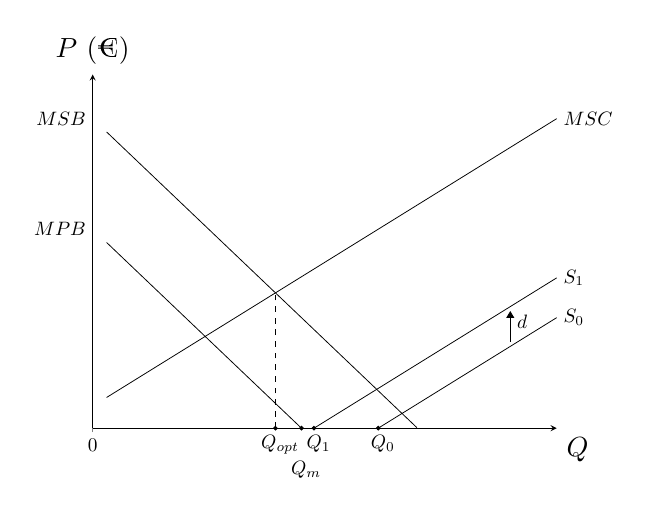
\begin{tikzpicture}[scale=0.7]
      \begin{axis}[
        width=10cm,
        height=8cm,
        axis lines = left,
        xtick = {0},
        ytick = {\empty},
        xmin = 0, xmax = 10,
        ymin = 0, ymax = 8,
        clip = false
      ]
      % Supply curves
      \addplot[domain = 0.3:10, restrict y to domain = 0:8, samples = 400]{0.65*x+0.5};
      \addplot[domain = 0.3:10, restrict y to domain = 0:8, samples = 400]{0.65*x-3.1};
      \addplot[domain = 0.3:10, restrict y to domain = 0:8, samples = 400]{0.65*x-4};

      % Demand curves
      \addplot[domain = 0.3:10, restrict y to domain = 0:8, samples = 400]{-x+4.5};
      \addplot[domain = 0.3:10, restrict y to domain = 0:8, samples = 400]{-x+7};

      % D/S curve labels
      \node[right] at (10, 7) {$MSC$};
      \node[right] at (10, 3.4) {$S_1$};
      \node[right] at (10, 2.5) {$S_0$};

      \node[left] at (0, 4.5) {$MPB$};
      \node[left] at (0, 7) {$MSB$};

      \draw[dashed] (3.939, 0) -- (3.939, 3.060);
      \filldraw[black] (3.939, 0) circle (1pt);
      \node[below] at (4.039, 0) {$Q_{opt}$};

      \filldraw[black] (4.5, 0) circle (1pt);
      \node[below] at (4.6, -0.6) {$Q_m$};

      \filldraw[black] (4.769, 0) circle (1pt);
      \node[below] at (4.869, 0) {$Q_1$};

      \filldraw[black] (6.154, 0) circle (1pt);
      \node[below] at (6.254, 0) {$Q_0$};

      \draw[-Triangle] (9, 1.95) to (9, 2.65);
      \node[right] at (9, 2.4) {$d$};



    \end{axis}
      \node[below right] at (current axis.right of origin) {$Q$};
      \node[above] at (current axis.above origin) {$P \text{ (\texteuro)}$};
    \end{tikzpicture}
    \caption{Remaining Welfare Loss}
  \end{center}
\end{wrapfigure}



\end{document}